\documentclass{beamer}\usepackage[]{graphicx}\usepackage[]{color}
%% maxwidth is the original width if it is less than linewidth
%% otherwise use linewidth (to make sure the graphics do not exceed the margin)
\makeatletter
\def\maxwidth{ %
  \ifdim\Gin@nat@width>\linewidth
    \linewidth
  \else
    \Gin@nat@width
  \fi
}
\makeatother

\definecolor{fgcolor}{rgb}{0.345, 0.345, 0.345}
\newcommand{\hlnum}[1]{\textcolor[rgb]{0.686,0.059,0.569}{#1}}%
\newcommand{\hlstr}[1]{\textcolor[rgb]{0.192,0.494,0.8}{#1}}%
\newcommand{\hlcom}[1]{\textcolor[rgb]{0.678,0.584,0.686}{\textit{#1}}}%
\newcommand{\hlopt}[1]{\textcolor[rgb]{0,0,0}{#1}}%
\newcommand{\hlstd}[1]{\textcolor[rgb]{0.345,0.345,0.345}{#1}}%
\newcommand{\hlkwa}[1]{\textcolor[rgb]{0.161,0.373,0.58}{\textbf{#1}}}%
\newcommand{\hlkwb}[1]{\textcolor[rgb]{0.69,0.353,0.396}{#1}}%
\newcommand{\hlkwc}[1]{\textcolor[rgb]{0.333,0.667,0.333}{#1}}%
\newcommand{\hlkwd}[1]{\textcolor[rgb]{0.737,0.353,0.396}{\textbf{#1}}}%
\let\hlipl\hlkwb

\usepackage{framed}
\makeatletter
\newenvironment{kframe}{%
 \def\at@end@of@kframe{}%
 \ifinner\ifhmode%
  \def\at@end@of@kframe{\end{minipage}}%
  \begin{minipage}{\columnwidth}%
 \fi\fi%
 \def\FrameCommand##1{\hskip\@totalleftmargin \hskip-\fboxsep
 \colorbox{shadecolor}{##1}\hskip-\fboxsep
     % There is no \\@totalrightmargin, so:
     \hskip-\linewidth \hskip-\@totalleftmargin \hskip\columnwidth}%
 \MakeFramed {\advance\hsize-\width
   \@totalleftmargin\z@ \linewidth\hsize
   \@setminipage}}%
 {\par\unskip\endMakeFramed%
 \at@end@of@kframe}
\makeatother

\definecolor{shadecolor}{rgb}{.97, .97, .97}
\definecolor{messagecolor}{rgb}{0, 0, 0}
\definecolor{warningcolor}{rgb}{1, 0, 1}
\definecolor{errorcolor}{rgb}{1, 0, 0}
\newenvironment{knitrout}{}{} % an empty environment to be redefined in TeX

\usepackage{alltt}


\mode<presentation>
{
\usetheme{Singapore}
\usecolortheme{dolphin}
%\useoutertheme{infolines}
\useoutertheme[subsection=false]{smoothbars}
%\useoutertheme[footline=authortitle, subsection=false]{miniframes}
\useinnertheme{circles}
\usefonttheme{structurebold}

\setbeamercovered{transparent}
}

\usepackage[english]{babel}
\usepackage{graphicx}
\usepackage{textcomp}
\usepackage{fancybox}
\usepackage{hyperref}
\usepackage{lmodern}
\usepackage{multirow}
\usepackage{booktabs}
\usepackage{array}
\usepackage{tipa}
\usepackage{caption}
\usepackage{float}
\usepackage{etoolbox}
\usepackage{ragged2e}
%\usepackage{enumitem}
\usepackage{setspace}
\usepackage{kotex}
\usepackage{tikz}
\usepackage{pgfpages}
\singlespacing

\usepackage{fontenc}
\usepackage[utf8]{inputenc}

\newcommand{\blue}[1]{{\color{blue}{#1}}}
\newcommand{\red}[1]{{\color{red}{#1}}}
\newcommand{\gray}[1]{{\color{gray}{#1}}}

\setbeamercolor{subtitle}{fg=gray}

\setbeamertemplate{note page}[plain]
%\setbeameroption{show notes on second screen=right} % both
\setbeameroption{hide notes} %only slidees
%\setbeameroption{show only notes} %Only notes


\makeatletter
\patchcmd{\beamer@sectionintoc}{\vskip1.5em}{\vskip0.5em}{}{}
\makeatother

%\addtobeamertemplate{frametitle}{}{%
%\begin{tikzpicture}[remember picture, overlay]
%\node[anchor=north east, yshift=-15pt] at (current page.north east)
%{\includegraphics[height=.69cm]{figure/Naver_clova_logo.pdf}};
%\end{tikzpicture}}

\title[LMM Tutorial]{A Tutorial for Linear models and Linear mixed effects models in R}

\subtitle[실험음성학연구회]{실험음성학연구회}

%\subtitle{X. Yang, X. Kong, M. Hasegawa-Johnson, and Y. Xie (2016) \\\textit{in Proc. of} Speech Prosody 2016, pp. 247--251.}

% - Use the \inst{?} command only if the authors have different
%   affiliation.
%\author{F.~Author\inst{1} \and S.~Another\inst{2}}
\author[Ryu et al.]{Hyuksu Ryu\inst{1}}

% - Use the \inst command only if there are several affiliations.
% - Keep it simple, no one is interested in your street address.
\institute[Naver Clova]{\inst{1} Naver Clova}
%\institute{NAVER Corporation, Seongnam, Korea}
\titlegraphic{
	
\includegraphics[height=.4cm]{../Naver_logo.pdf}
	\hspace*{3cm}
	\includegraphics[height=.5cm]{../Naver_clova_logo.pdf}
	}

\date{August 11, 2017}



% If you have a file called "university-logo-filename.xxx", where xxx
% is a graphic format that can be processed by latex or pdflatex,
% resp., then you can add a logo as follows:

% \pgfdeclareimage[height=0.5cm]{university-logo}{university-logo-filename}
% \logo{\pgfuseimage{university-logo}}



% Delete this, if you do not want the table of contents to pop up at
% the beginning of each subsection:
\AtBeginSection[]
{
\begin{frame}<beamer>
\frametitle{Outlines}
\tableofcontents[currentsection, hideallsubsections]
%\tableofcontents[currentsection]
\end{frame}
}
\IfFileExists{upquote.sty}{\usepackage{upquote}}{}
\begin{document}



\begin{frame}
\maketitle
\end{frame}

\begin{frame}
\frametitle{T.O.C}
	\tableofcontents[subsectionstyle=hide]
\end{frame}

\section{Instruction}
\subsection{Instruction}

\begin{frame}
\frametitle{Instruction}
What we are dealing with?
\begin{enumerate}
\item \alert{Linear model} $\quad \leftarrow$
\item Linear mixed model
\end{enumerate}
\end{frame}

\section{Example Description}
\subsection{Example Description}

\begin{frame}
\frametitle{Example description}
Question
\begin{itemize}
\item Assume you knew nothing about males and females
\item you were interested in whether \alert{voice pitch} of males and females differs, if so, by how much
\end{itemize}

\vspace{9pt}
Experiment
\begin{itemize}
\item take a bunch of males and females
\item ask them to say a single word
\item measure the respective voice pitches
\end{itemize}

\end{frame}

\begin{frame}
\frametitle{Example description}

\begin{center}
\begin{tabular}{ccc}
\toprule
\texttt{Subject} & \texttt{Sex} & \texttt{Voice.Pitch(Hz)} \\
\midrule
1 & female & 233 \\
2 & female & 204 \\
3 & female & 242 \\
4 & male & 130 \\
5 & male & 112 \\
6 & male & 142 \\
\bottomrule
\end{tabular}
\end{center}

\end{frame}

\begin{frame}
\frametitle{Example description}
It looks like
\begin{itemize}
\item the female values seem to be about 100 Hz above the male ones
\item females have higher voice pitch than males
\end{itemize}

\vspace{9pt}
But
\begin{itemize}
\item it could be the case that females and males have the same pitch
\item you were just unlucky and happened to choose some exceptionally high-pitched females and some exceptionally low-pitched males
\end{itemize}
\end{frame}

\begin{frame}
\frametitle{Example description}
We might want
\begin{itemize}
\item a more precise estimate of the difference between males and females
\item an estimate about how likely (or unlikely) that difference in voice pitch could have arisen just because of drawing an unlucky sample
\end{itemize}

$\rightarrow$ \alert{The linear model} comes in
\begin{itemize}
\item give some value about voice pitch for males and females
\item as well as \alert{some probability values} as to how likely those values are
\end{itemize}
\end{frame}

\begin{frame}[fragile]
\frametitle{Example description}
Basic idea
\begin{itemize}
\item relationship b/w sex and voice pitch as a simple formula
\item \verb|pitch ~ sex|
\item This reads
	\begin{itemize}
	\item pitch predicted by sex
	\item pitch as a function of sex
	\end{itemize}
\item LEFT: \texttt{pitch}
	\begin{itemize}
	\item dependent variable
	\item the thing you measure
	\end{itemize}
\item RIGHT: \texttt{sex}
	\begin{itemize}
	\item independent variable
	\item explanatory variable
	\item predictor
	\end{itemize}
\end{itemize}
\end{frame}

\begin{frame}[fragile]
\frametitle{Example Description}
Error term
\begin{itemize}
\item Problem: the world is not perfect.
\item Pitch is not \textit{completely} determined by sex
\item a bunch of different factors such as language, dialect, etc
\item We can never measure and control all of these things
\item update our formula to capture the existence of these ``random'' factors.
\item \verb|pitch ~ sex| + $\epsilon$ 
\item $\epsilon$
	\begin{itemize}
	\item an error term
	\item stands for all of the things that affect pitch that are not sex,
	\item all of the stuff that is random or uncontrollable
	\end{itemize}
\end{itemize}

\end{frame}

\section[Exercise1]{Exercise 1: Pitch $\sim$ Sex}
\subsection{Exercise}

\begin{frame}[fragile]
\frametitle{Exercise}
Let's create the dataset
\begin{knitrout}
\definecolor{shadecolor}{rgb}{0.969, 0.969, 0.969}\color{fgcolor}\begin{kframe}
\begin{alltt}
\hlstd{pitch} \hlkwb{=} \hlkwd{c}\hlstd{(}\hlnum{233}\hlstd{,}\hlnum{204}\hlstd{,}\hlnum{242}\hlstd{,}\hlnum{130}\hlstd{,}\hlnum{112}\hlstd{,}\hlnum{142}\hlstd{)}
\hlstd{sex} \hlkwb{=} \hlkwd{c}\hlstd{(}\hlkwd{rep}\hlstd{(}\hlstr{"female"}\hlstd{,}\hlnum{3}\hlstd{),}\hlkwd{rep}\hlstd{(}\hlstr{"male"}\hlstd{,}\hlnum{3}\hlstd{))}
\hlstd{my.df} \hlkwb{=} \hlkwd{data.frame}\hlstd{(sex, pitch)}
\end{alltt}
\end{kframe}
\end{knitrout}

\pause

\begin{knitrout}
\definecolor{shadecolor}{rgb}{0.969, 0.969, 0.969}\color{fgcolor}\begin{kframe}
\begin{alltt}
\hlstd{my.df}
\end{alltt}
\begin{verbatim}
##      sex pitch
## 1 female   233
## 2 female   204
## 3 female   242
## 4   male   130
## 5   male   112
## 6   male   142
\end{verbatim}
\end{kframe}
\end{knitrout}
\end{frame}

\begin{frame}[fragile]
\frametitle{Exercise}
\begin{itemize}
\item \texttt{lm()}
	\begin{itemize}
	\item Generate the linear model
	\item Note that we omit the ``$\epsilon$'' term 
	\item we saved the model into an object \texttt{xmdl}
	\end{itemize}
\pause
\begin{knitrout}
\definecolor{shadecolor}{rgb}{0.969, 0.969, 0.969}\color{fgcolor}\begin{kframe}
\begin{alltt}
\hlstd{xmdl} \hlkwb{=} \hlkwd{lm}\hlstd{(pitch} \hlopt{~} \hlstd{sex, my.df)}
\end{alltt}
\end{kframe}
\end{knitrout}
\end{itemize}
\end{frame}

\begin{frame}[fragile]
\frametitle{Exercise}
\begin{itemize}

\item \texttt{summary()}
	\begin{itemize}
	\item To see what the linear model did
	\end{itemize}
\begin{knitrout}
\definecolor{shadecolor}{rgb}{0.969, 0.969, 0.969}\color{fgcolor}\begin{kframe}
\begin{alltt}
\hlkwd{summary}\hlstd{(xmdl)}
\end{alltt}
\end{kframe}
\end{knitrout}
\end{itemize}
\end{frame}


\begin{frame}[fragile]
\frametitle{Exercise}

\begin{columns}[T]
\begin{column}{.7\textwidth}
\begin{knitrout}\tiny
\definecolor{shadecolor}{rgb}{0.969, 0.969, 0.969}\color{fgcolor}\begin{kframe}
\begin{verbatim}
## 
## Call:
## lm(formula = pitch ~ sex, data = my.df)
## 
## Residuals:
##       1       2       3       4       5       6 
##   6.667 -22.333  15.667   2.000 -16.000  14.000 
## 
## Coefficients:
##             Estimate Std. Error t value Pr(>|t|)    
## (Intercept)   226.33      10.18  22.224 2.43e-05 ***
## sexmale       -98.33      14.40  -6.827  0.00241 ** 
## ---
## Signif. codes:  0 '***' 0.001 '**' 0.01 '*' 0.05 '.' 0.1 ' ' 1
## 
## Residual standard error: 17.64 on 4 degrees of freedom
## Multiple R-squared:  0.921,	Adjusted R-squared:  0.9012 
## F-statistic: 46.61 on 1 and 4 DF,  p-value: 0.002407
\end{verbatim}
\end{kframe}
\end{knitrout}
\end{column}
\begin{column}{.35\textwidth}
\vspace{15pt}
$\leftarrow$ the model formula you entered 

$\leftarrow$ the residuals

\vspace{14pt}
$\leftarrow$ the coefficients of the fixed effects

\vspace{18pt}
$\leftarrow$ the output prints some overall results of the model
\end{column}
\end{columns}
\end{frame}

\begin{frame}
\frametitle{Output}
Multiple R-Squared
\begin{itemize}
\item $R^2$ 
	\begin{itemize}
	\item variance explained
	\item variance accounted for
	\item 0.921 (quite high) means 92.1\% of the stuff is ``explained'' by our model
	\end{itemize}
\item In this case, we have only one independent variable (the fixed effect ``sex''),
\item $R^2$ reflects how much variance in our data is accounted for by \alert{differences b/w males and females}
\item In general, b/c $R^2$ value depends on how messy or complex the system is
\item frequently deal with much lower $R^2$ values. 
\end{itemize}
\end{frame}


\begin{frame}
\frametitle{Output}
Multiple R-Squared and Adjusted R-squared
\begin{itemize}
\item If you have two or more variables (fixed effect), you see Adjusted R-squared ($R^2_{adj}$), instead of Multiple R-squared.
\item $R^2$ has a property that it is increased when variables are added up, even though the variables are irrelevant.
\item ``Adjusted'' R-squared are adjusted considering how many fixed effects you used.
\end{itemize}
\end{frame}

\begin{frame}
\frametitle{Output}
Meaning of p-value in the F-statistics
\begin{itemize}
\item \textbf{conditional probability}
\item a probability \textit{under the condition that the $H_0$ is true}
\item $H_0$: sex has no effect on pitch
\item ``statistically significant'' when the conditional probability is lower than a threshold, adn the alternative hypothesis ($H_1$) is more likely.
\item Report
	\begin{itemize}
	\item ``We constructed a linear model of pitch as a function of sex. This model was significnat (F(1,4)=46.61, p$>$0.01).''
	\end{itemize}

\vspace{9pt}
\item How to distinguish b/w the significance of the overall model (considering all effects together) from the p-value of individual coefficients? $\rightarrow$ to be continue
\end{itemize}
\end{frame}

\begin{frame}[fragile]
\frametitle{output}
Coefficients table
\begin{knitrout}\scriptsize
\definecolor{shadecolor}{rgb}{0.969, 0.969, 0.969}\color{fgcolor}\begin{kframe}
\begin{verbatim}
##              Estimate Std. Error   t value     Pr(>|t|)
## (Intercept) 226.33333   10.18441 22.223508 2.426952e-05
## sexmale     -98.33333   14.40293 -6.827314 2.406892e-03
\end{verbatim}
\end{kframe}
\end{knitrout}
\begin{itemize}
\item Compare p-value for the overall model and that on the right-hand side of the coefficients table
\item Same b/c the model had only one fixed effect
\end{itemize}
\end{frame}

\begin{frame}[fragile]
\frametitle{output}
Coefficients table
\begin{knitrout}\scriptsize
\definecolor{shadecolor}{rgb}{0.969, 0.969, 0.969}\color{fgcolor}\begin{kframe}
\begin{verbatim}
##              Estimate Std. Error   t value     Pr(>|t|)
## (Intercept) 226.33333   10.18441 22.223508 2.426952e-05
## sexmale     -98.33333   14.40293 -6.827314 2.406892e-03
\end{verbatim}
\end{kframe}
\end{knitrout}
\begin{itemize}
\item Why \texttt{sexmale}, rather than just \texttt{sex}?
	\begin{itemize}
	\item Estimate of \texttt{intercept}: mean of pitch of female 
	\item Estimate of \texttt{sexmale}: difference of pitch b/w female and male
	\item $\therefore$ pitch of male = Estimate of \texttt{intercept} + Estimate of \texttt{sexmale}
	\end{itemize}

\vspace{9pt}
\begin{center}
\begin{tabular}{cccc}

\toprule
& female & male & difference \\
\midrule
mean & 226.333 & 128 & 98.333 \\
\bottomrule
\end{tabular}
\end{center}
\end{itemize}
\end{frame}

\begin{frame}[fragile]
\frametitle{output}
Graphical interpretation
\begin{knitrout}
\definecolor{shadecolor}{rgb}{0.969, 0.969, 0.969}\color{fgcolor}
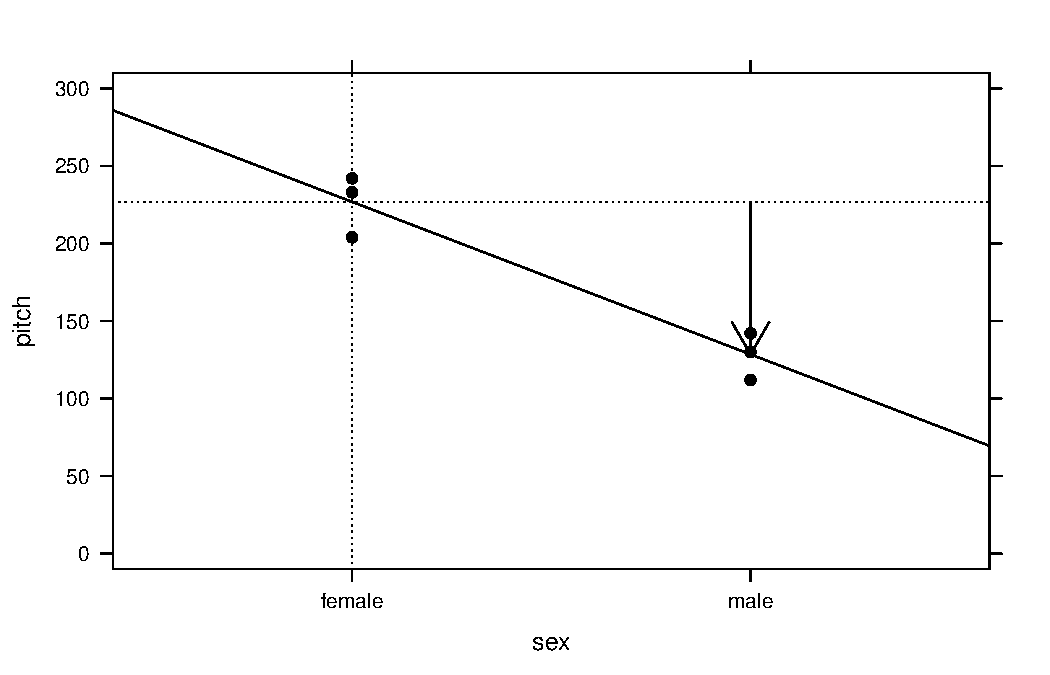
\includegraphics[width=\maxwidth]{figure/unnamed-chunk-9-1} 

\end{knitrout}
\end{frame}
\begin{frame}
\frametitle{output}
Secret of Intercept: Why did the model choose females to be the intercept?
\pause

\vspace{9pt}
$\because$ \texttt{lm()} function simply takes whatever comes first in \alert{alphabet} 

``f'' comes before ``m''

\end{frame}

\section[Exercise2]{Exercise 2: Pitch $\sim$ Age}
\subsection[Ex2]{Exercise2}

\begin{frame}[fragile]
\frametitle{New model}
Whether age predicts voice pitch
\begin{itemize}
\item continuous as explanatory 
\item pitch $\sim$ age + $\epsilon$
\end{itemize}
\begin{center}
\begin{tabular}{ccc}
\toprule
Subject & Age & Pitch(Hz) \\
\midrule
1 & 14 & 252 \\
2 & 23 & 244 \\
3 & 35 & 240 \\
4 & 48 & 233 \\
5 & 52 & 212 \\
6 & 67 & 204 \\
\bottomrule
\end{tabular}
\end{center}
\end{frame}

\begin{frame}[fragile]
\frametitle{output}
\begin{knitrout}\tiny
\definecolor{shadecolor}{rgb}{0.969, 0.969, 0.969}\color{fgcolor}\begin{kframe}
\begin{alltt}
\hlstd{age} \hlkwb{=} \hlkwd{c}\hlstd{(}\hlnum{14}\hlstd{,}\hlnum{23}\hlstd{,}\hlnum{35}\hlstd{,}\hlnum{48}\hlstd{,}\hlnum{52}\hlstd{,}\hlnum{67}\hlstd{)}
\hlstd{pitch} \hlkwb{=} \hlkwd{c}\hlstd{(}\hlnum{252}\hlstd{,}\hlnum{244}\hlstd{,}\hlnum{240}\hlstd{,}\hlnum{233}\hlstd{,}\hlnum{212}\hlstd{,}\hlnum{204}\hlstd{)}
\hlstd{my.df} \hlkwb{=} \hlkwd{data.frame}\hlstd{(age, pitch)}
\hlstd{xmdl} \hlkwb{=} \hlkwd{lm}\hlstd{(pitch}\hlopt{~}\hlstd{age, my.df)}
\hlkwd{summary}\hlstd{(xmdl)}
\end{alltt}
\begin{verbatim}
## 
## Call:
## lm(formula = pitch ~ age, data = my.df)
## 
## Residuals:
##      1      2      3      4      5      6 
## -2.338 -2.149  4.769  9.597 -7.763 -2.115 
## 
## Coefficients:
##             Estimate Std. Error t value Pr(>|t|)    
## (Intercept) 267.0765     6.8522   38.98 2.59e-06 ***
## age          -0.9099     0.1569   -5.80  0.00439 ** 
## ---
## Signif. codes:  0 '***' 0.001 '**' 0.01 '*' 0.05 '.' 0.1 ' ' 1
## 
## Residual standard error: 6.886 on 4 degrees of freedom
## Multiple R-squared:  0.8937,	Adjusted R-squared:  0.8672 
## F-statistic: 33.64 on 1 and 4 DF,  p-value: 0.004395
\end{verbatim}
\end{kframe}
\end{knitrout}
\end{frame}

\begin{frame}[fragile]
\frametitle{output}
Coefficient table
\begin{knitrout}\scriptsize
\definecolor{shadecolor}{rgb}{0.969, 0.969, 0.969}\color{fgcolor}\begin{kframe}
\begin{verbatim}
##                Estimate Std. Error   t value     Pr(>|t|)
## (Intercept) 267.0764640  6.8521942 38.976780 2.588356e-06
## age          -0.9098694  0.1568771 -5.799888 4.394969e-03
\end{verbatim}
\end{kframe}
\end{knitrout}
\begin{itemize}
\item the significance of the intercept is NOT important
	\begin{itemize}
	\item intercept means predicted pitch for people with age 0
	\end{itemize}
\item the significance of the age IS real interest.
	\begin{itemize}
	\item every increase of age by 1 $\rightarrow$ decrease voice pitch by 0.9099
	\end{itemize}

\end{itemize}
\end{frame}

\begin{frame}[fragile]
\frametitle{output}
Graphical interpretation
\begin{knitrout}
\definecolor{shadecolor}{rgb}{0.969, 0.969, 0.969}\color{fgcolor}
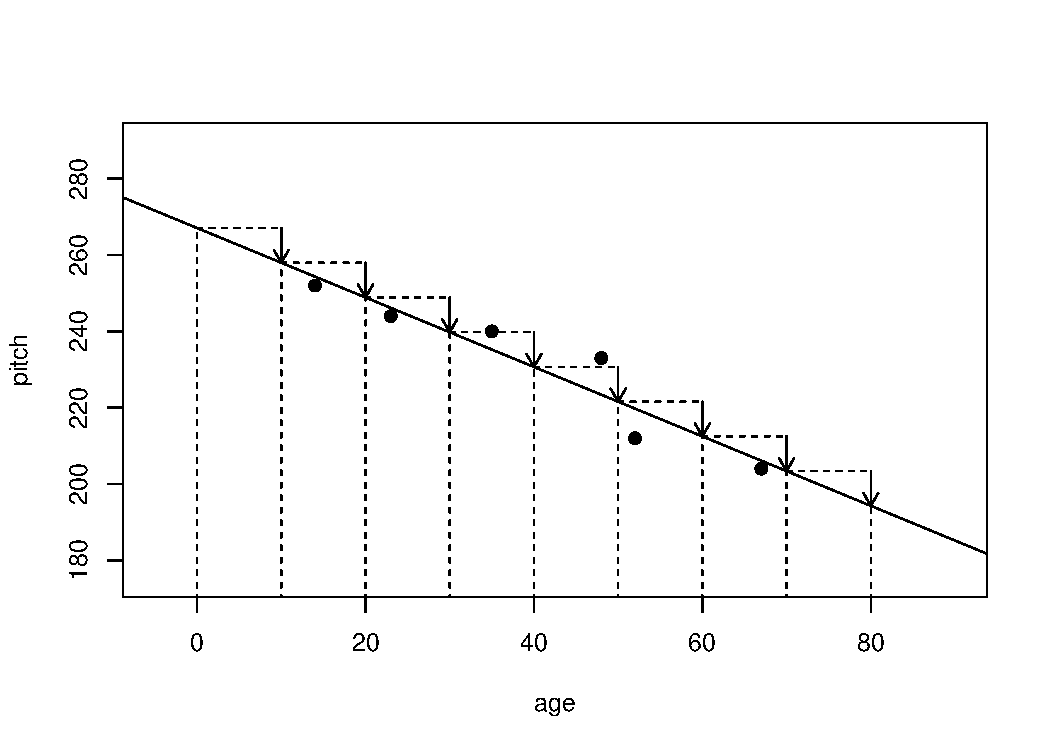
\includegraphics[width=\maxwidth]{figure/unnamed-chunk-12-1} 

\end{knitrout}

\end{frame}

\begin{frame}[fragile]
\frametitle{output}
Meaningful and meaningless intercepts
\begin{knitrout}
\definecolor{shadecolor}{rgb}{0.969, 0.969, 0.969}\color{fgcolor}\begin{kframe}
\begin{alltt}
\hlstd{my.df}\hlopt{$}\hlstd{age.c} \hlkwb{=} \hlstd{my.df}\hlopt{$}\hlstd{age} \hlopt{-} \hlkwd{mean}\hlstd{(my.df}\hlopt{$}\hlstd{age)}
\hlstd{xmdl} \hlkwb{=} \hlkwd{lm}\hlstd{(pitch}\hlopt{~}\hlstd{age.c, my.df)}
\end{alltt}
\end{kframe}
\end{knitrout}
\begin{itemize}
\item new column ``age.c'' $\rightarrow$ ``centered'' data
\begin{knitrout}\scriptsize
\definecolor{shadecolor}{rgb}{0.969, 0.969, 0.969}\color{fgcolor}\begin{kframe}
\begin{verbatim}
##                Estimate Std. Error   t value     Pr(>|t|)
## (Intercept) 230.8333333  2.8112916 82.109353 1.318716e-07
## age.c        -0.9098694  0.1568771 -5.799888 4.394969e-03
\end{verbatim}
\end{kframe}
\end{knitrout}
\item Same slope, but \alert{different} intercept
\item intercept here means pitch at mean age $\rightarrow$ mean pitch
\item intercept becomes more meaningful than previous
\end{itemize}
\end{frame}

\begin{frame}
\frametitle{Going on}
Scaling up
\begin{itemize}
\item What if we measured two factors, such as age and sex?
\item Multiple regression
	\begin{itemize}
	\item one response variable as a function of multiple predictor variables
	\item linear model is just another word for multiple regression
	\end{itemize}
\item formula
\begin{displaymath}
pitch \sim sex + age + \epsilon
\end{displaymath}
\item But, same interpretation
\item The p-value at the bottom of the output
	\begin{itemize}
	\item p-value for the \alert{overall model}
	\item p-value considers how well all of your fixed effects together help in accounting for variation in pitch
	\end{itemize}
\item The coefficient output
	\begin{itemize}
	\item p-value for the individual fixed effects
	\end{itemize}
\end{itemize}
\end{frame}

\begin{frame}
\frametitle{The end of Linear model}
\centering
\Huge
The end of linear model!

But one more thing!
\end{frame}

\section{Assumption}
\subsection{Assumptions}
\begin{frame}
\frametitle{Assumptions for LM}
Assumptions for applying a linear model
\begin{enumerate}
\item Linearity
\item Absense of collinearity
\item Homoskedasticity
\item Normality of residuals
\item Absense of influential data points
\item Independence
\end{enumerate}
\end{frame}

\subsection{Linearity}
\begin{frame}
\frametitle{Linearity}
Linearity?
\begin{itemize}
\item linear what?
\pause
\item linearity of residuals
\pause
\item So, what is residuals?
\end{itemize}
\end{frame}

\begin{frame}[fragile]
\frametitle{Linearity}
Residuals
\begin{itemize}
\item Deviations of the observed data points from the predicted values (fitted values)
\item In this case, the residuals very small $\rightarrow$ well predicted
\end{itemize}

\begin{knitrout}
\definecolor{shadecolor}{rgb}{0.969, 0.969, 0.969}\color{fgcolor}
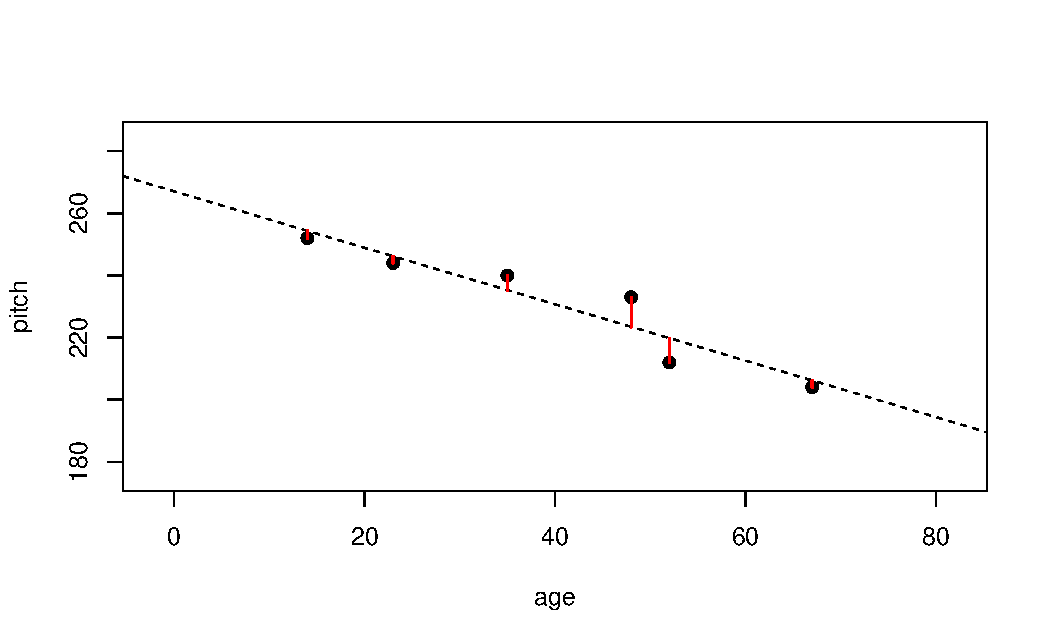
\includegraphics[width=\maxwidth]{figure/unnamed-chunk-15-1} 

\end{knitrout}
\end{frame}

\begin{frame}[fragile]
\frametitle{Linearity}
Residuals
\begin{itemize}
\item Rotate the plot $\rightarrow$ Residual plot

\begin{knitrout}\footnotesize
\definecolor{shadecolor}{rgb}{0.969, 0.969, 0.969}\color{fgcolor}\begin{kframe}
\begin{alltt}
\hlkwd{plot}\hlstd{(}\hlkwd{fitted}\hlstd{(xmdl),} \hlkwd{residuals}\hlstd{(xmdl),}\hlkwc{pch}\hlstd{=}\hlnum{19}\hlstd{,}
        \hlkwc{xlab} \hlstd{=} \hlstr{'Fitted values'}\hlstd{,} \hlkwc{ylab}\hlstd{=}\hlstr{'Residuals'} \hlstd{)}
\end{alltt}
\end{kframe}
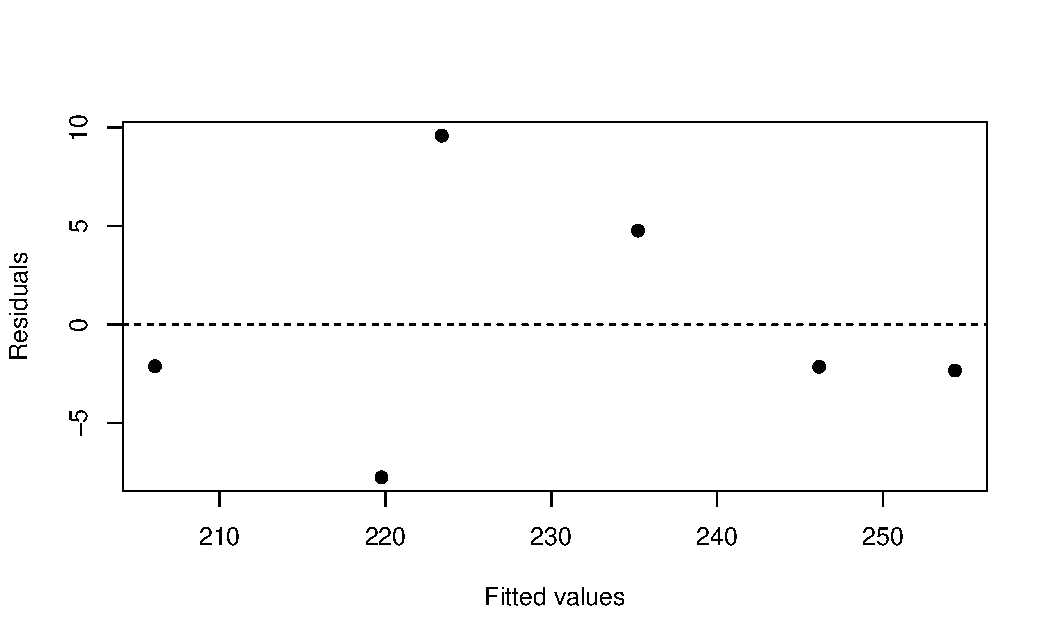
\includegraphics[width=\maxwidth]{figure/residual_plot-1} 

\end{knitrout}

\end{itemize}
\end{frame}

\begin{frame}
\frametitle{Linearity}
Residual plot
\begin{itemize}
\item The fitted values - on the horizontal line
\item residuals - the vertical deviations from the line
\item \alert{No obvious pattern} in the residuals $\rightarrow$ \textbf{Linear}
\pause
\item What if there were a nonlinear or curvy pattern?
\item this would indicate a violation of the linearity assumption
\end{itemize}
\begin{center}
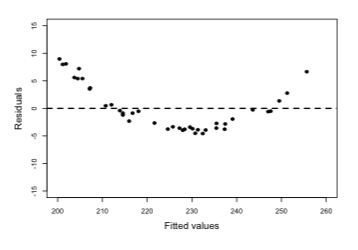
\includegraphics[scale=.4]{figure/fig1}
\end{center}
\end{frame}

\begin{frame}
\frametitle{Linearity}
What to do in case of non-linearity?
\begin{enumerate}
\item You might miss an important fixed effects. Add them
\item Perform a \alert{nonlinear transformation} of your response, e.g., log-transform (\textit{commonly chosen})
\item Perfrom a nonlinear transformation of your fixed effects
	\begin{itemize}
	\item if \textit{age} showed in a U-shaped
	\item add age and $age^2$ as predictors
	\end{itemize}	
\item if stripes in residual plot, then you're most likely dealing with \alert{categorical data} $\rightarrow$ different model such as logistic models
\end{enumerate}
\begin{center}
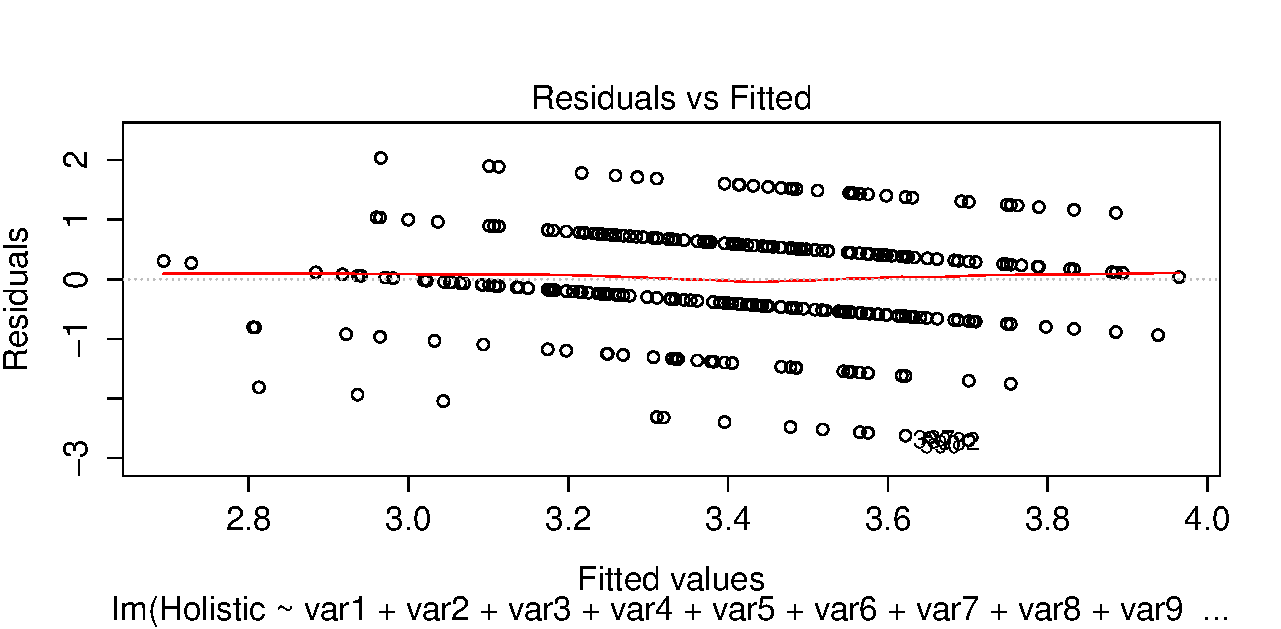
\includegraphics[scale=.3]{figure/stripe}
\end{center}
\end{frame}

\subsection{Collinearity}
\begin{frame}
\frametitle{Collinearity}
What is collinearity?
\begin{itemize}
\item When two fixed effects (predictors) are \alert{correlated with} each other,
\item they are said to be \textbf{collinear}
\end{itemize}

Example
\begin{itemize}
\item you were interested in how average talking speed affects intellignece ratings
\begin{displaymath}
intelligence\ ratings \sim talking\ speed
\end{displaymath}
\item you measured several different indicators of talking speed
	\begin{itemize}
	\item syllables/sec, words/sec, sentences/sec
	\end{itemize}
\item they are likely to be highly correlated with each other
\item if you use all of them as predictors within the same model, there will be \textbf{collinearity problem}
\end{itemize}
\end{frame}

\begin{frame}
\frametitle{Collinearity}
If there is collinearity
\begin{itemize}
\item the interpretation of the model becomes \alert{unstable}
\item the significance of these correlated or collinear fixed effects is not easily interpretable
\begin{itemize}
\item $\because$ they might steal each other's \alert{explanatory power}
\end{itemize}
\item if multiple predictors are very similar to each other
	\begin{itemize}
	\item it becomes very difficult to decide what, in fact, is playing a big role
	\end{itemize}
\end{itemize}
\end{frame}

\begin{frame}
\frametitle{Collinearity}
How to get rid of collinearity?
\begin{enumerate}
\item pre-empt the problem in the design stage
	\begin{itemize}
	\item focus on a few fixed effects that are not correlated with each other
	\end{itemize}
\item Or, think about which one is the most meaningful and drop the others
	\begin{itemize}
	\item DO NOT base this dropping decision on the \textbf{significance} (circular logic problem)
	\end{itemize}
\item Or, consider dimension-reduction techniques such as Principal Component Analysis
	\begin{itemize}
	\item transform several correlated variables into a smaller set of variables which you can then use as new fixed effects.
	\end{itemize}
\end{enumerate}
\end{frame}

\subsection{Homoskedasticity}
\begin{frame}
\frametitle{Homoskedasticity}
What is Homoskedasticity?
\begin{itemize}
\item The variance of your data should be approximately equal across the range of your predicted values
\item it is \textbf{extremely important assumption}
\item If homoscedasticiy is violated $\rightarrow$ a problem with unequal variances
\end{itemize}
\end{frame}

\begin{frame}
\frametitle{Homoskedasticity}
How to check whether homoscedasticity assumption were met?
\begin{itemize}
\item the \textbf{residuals} of your model need to roughly have a similar amount of deviation from the predicted values
\item See Residual Plot
\item Good residual plot essentially looks blob-like
\end{itemize}
\begin{knitrout}
\definecolor{shadecolor}{rgb}{0.969, 0.969, 0.969}\color{fgcolor}
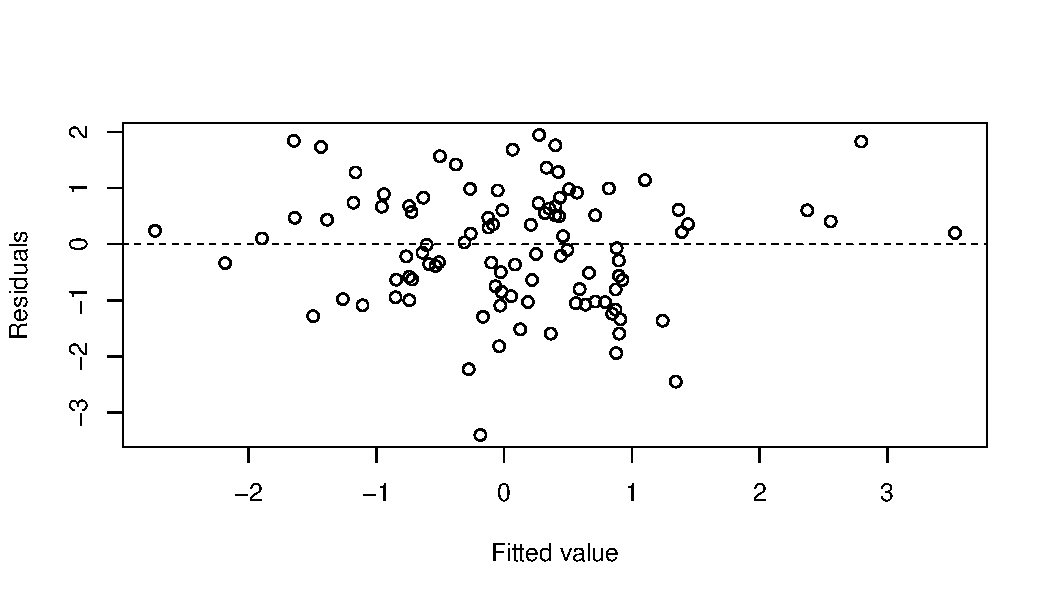
\includegraphics[width=\maxwidth]{figure/unnamed-chunk-16-1} 

\end{knitrout}

\end{frame}


\begin{frame}
\frametitle{Homoskedasticity}
Example of \textbf{heteroskedasticity}
\begin{center}
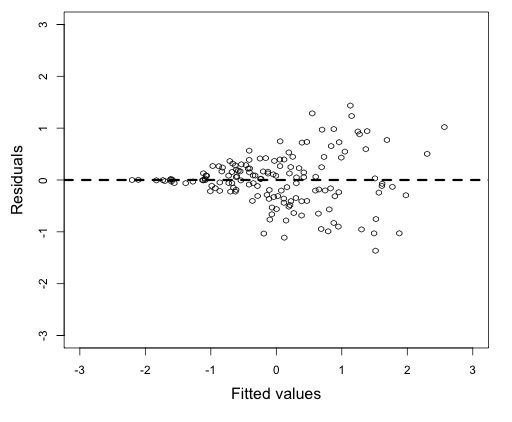
\includegraphics[scale=.25]{figure/fig2}
\end{center}
\begin{itemize}
\item higher fitted values have larger residuals
\end{itemize}

What to do?
\begin{itemize}
\item As mentioned earlier, consider a \alert{log-transform}
\end{itemize}
\end{frame}

\subsection{Normality of residuals}
\begin{frame}
\frametitle{Normality of residuals}
Normality of residuals
\begin{itemize}
\item It is the one that is \alert{least important}
\item LM is relatively robust agains violation of the normality assumption
\item Gellman and Hill (2007), a famous book on LM and mixed models, DO NOT EVEN RECOMMEND diagnostics of the normality assumption
\end{itemize}

If you want to test the assumption
\begin{itemize}
\item Histogram
\begin{knitrout}\scriptsize
\definecolor{shadecolor}{rgb}{0.969, 0.969, 0.969}\color{fgcolor}\begin{kframe}
\begin{alltt}
\hlkwd{hist}\hlstd{(}\hlkwd{residuals}\hlstd{(xmdl))}
\end{alltt}
\end{kframe}
\end{knitrout}
\item Q-Q plot
\begin{knitrout}\scriptsize
\definecolor{shadecolor}{rgb}{0.969, 0.969, 0.969}\color{fgcolor}\begin{kframe}
\begin{alltt}
\hlkwd{qqnorm}\hlstd{(}\hlkwd{residuals}\hlstd{(xmdl))}
\end{alltt}
\end{kframe}
\end{knitrout}
\end{itemize}
\end{frame}

\begin{frame}
\frametitle{Normality of residuals}
Example of normality
\begin{center}
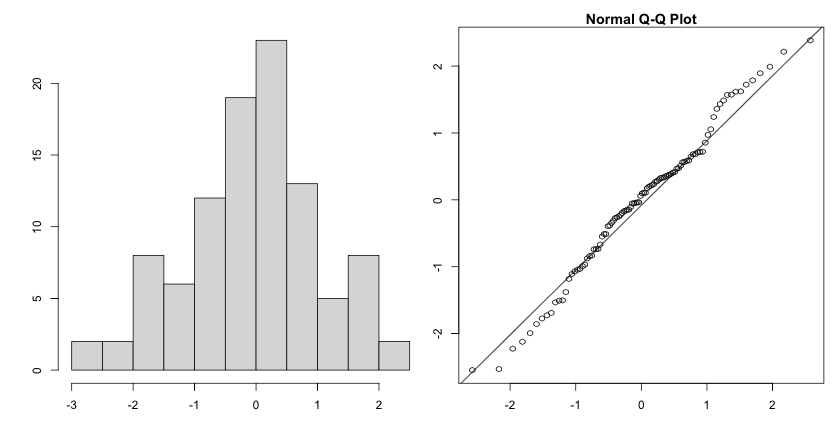
\includegraphics[scale=.2]{figure/fig3}
\end{center}
\begin{itemize}
\item Thses look good
\item The histogram is relatively bell-shaped
\item The Q-Q plot indicates that the data falls on a straight line
	\begin{itemize}
	\item which means that it's similar to a normal distribution
	\end{itemize}
\item can conclude that there are no obvious violations of the normalitry assumption
\end{itemize}
\end{frame}

\subsection{Absence of influential data points}
\begin{frame}
\frametitle{Absence of influential data points}
What is the influential data point?
\begin{itemize}
\item If a particular data point is excluded, when values with which the coefficient is adjusted is large, it is an influential data point.
\item Influential data points can drastically change the interpretation of the results, it can lead to instable results
\end{itemize}
\end{frame}

\begin{frame}[fragile]
\frametitle{Absence of influential data points}
How to check?
\begin{itemize}
\item Using \texttt{dfbeta()} function
\begin{knitrout}\scriptsize
\definecolor{shadecolor}{rgb}{0.969, 0.969, 0.969}\color{fgcolor}\begin{kframe}
\begin{alltt}
\hlkwd{dfbeta}\hlstd{(xmdl)}
\end{alltt}
\begin{verbatim}
##   (Intercept)         age
## 1  -3.3645662  0.06437573
## 2  -1.6119656  0.02736278
## 3   1.5481303 -0.01456709
## 4  -0.0259835  0.05092767
## 5   0.8707699 -0.06479736
## 6   1.8551808 -0.06622744
\end{verbatim}
\end{kframe}
\end{knitrout}
\item DFbeta values are the values of coefficient as a result of \textit{leave-one-out diagnostics}
\item For example, if data point 1 is excluded, the coefficient for age has to be adjsted by 0.0644 from -0.9099, so -0.8455
\end{itemize}
\end{frame}

\begin{frame}
\frametitle{Absence of influential data points}
What is the criteria for decision of influential data point
\begin{itemize}
\item There is no clear, sharp criteria
\item One thing for sure
	\begin{itemize}
	\item any value that changes the sign of the slope is \textbf{definitely} an influential point
	\item be cautious to DFbeta value which is at least half of the absolute value of the slope (To author)
	\end{itemize}
\end{itemize}
\end{frame}

\begin{frame}
\frametitle{Absence of influential data points}
How to proceed if there are influential data points?
\begin{itemize}
\item DO NOT SIMPLY EXCLUDE those points and report only the results on the reduced set
	\begin{itemize}
	\item The only case to exclude influential points is when
	\item there is an obvious error (negative age)
	\item or there is a value that obviously is the result due to a technical error (voice pitch value of 0)
	\end{itemize}
\item Run the analysis \textbf{with} the influential points and \textbf{without} the points, reports both analyses, state whether the interpretation of the results does or does not change 
\end{itemize}
\end{frame}

\subsection{Independence}
\begin{frame}
\frametitle{Independence}
What is independence?
\begin{itemize}
\item easy example - coin flip or roll of a dice
\item each try is not influenced by another try
\item each coin flip and each roll of a dice is absolutely independent from the outcome of the preceding coin flips or dice rolls
\item The same should hold for your data points for LM analysis
\item \alert{the data points should come from DIFFERENT SUBJECT}
\item Each subject should only contribute one data point
\item Independence assumption is by far \textbf{the most important one}
\end{itemize}
\end{frame}


\begin{frame}
\frametitle{Independence}
When you violate the indepence assumption?
\begin{itemize}
\item may greatly inflate chance of finding a \textit{spurious result}
\item and it results in a p-value that is \textit{completely meaningless}.
\end{itemize}

How can guarantee independence?
\begin{itemize}
\item Independence is a \textbf{question of the experimental design}
\item by only collecting one data point per subject
\end{itemize}
\end{frame}

\begin{frame}
\frametitle{Independence}
If you want to collect more data per subject?
\begin{itemize}
\item such as in repreated measures design
\item need to resolve these non-independence at the analysis stage
\item This is where \textbf{MIXED MODELS} comes in
\end{itemize}
\pause
\begin{center}
\huge
Mixed models will be proceeded in Tutorial 2
\end{center}
\end{frame}


\end{document}
